\setcounter{chapter}{ 19 }
\chapter{\textbf{``Smooth Operator''} }




\subChapterTitle{(Borrough Station ver 1.0)}

\deets{Suko}{May 6th, 2013}



New promotions!  New guns!  Lackovich in peril!  Arch nemesis lurking!



NOTE: I got sick of typing ``\_\_\_ thought'' or the even clunkier ``\_\_\_\_ thought to \_\_\_\_'' and the overlapping speech/thinking was getting complicated.  So I just color coded the thoughts:  \jayaBrain{Jaya}, \hayleyBrain{Hayley},  \oliverBrain{Oliver} ,  \jonahBrain{Jonah}\footnote{\textbf{Rebecca (as editor) }Suko came up with excellent colors for the characters- Jaya (red), Hayley (orange), Oliver (green), Jonah (blue). Unfortunately they don't print well in black \& white. So symbols were selected \& the colors retained but severely darkened so the text was readable.}
  without attribution.  We just have to remember who can hear which thoughts.  Hope that makes sense to people.  If it's unreadable, say so and I'll try something else.  At least it's more colorful.



NOTE \#2: The last few scenes (post-instrumentation) are going to be really patchy on details and dialog, especially between Jaya and Jonah.  Please please fill in what you recall.  Danke!




\jumpHeadline{SAC-09}

After meeting up with Octavia, Hayley goes to see Signe and gains a lot of emotional equilibrium back.  Jonah goes to investigate into his sister's new boyfriend.  Oliver and Jaya are the first to return to the base.



SAC-09 is in a flurry of activity and they are told to stay in their quarters as much as possible.  Micah is directing the movement of various supplies and equipment.  Lackovich is still absent, so Oliver hangs out with Patrol Group 2 again (who were also restricted to their barracks).



Jonah and Hayley return also, and are back for less than a day when Rook stops by and says that there will be a briefing in one hour.  Hayley does her very best to get them there early.   Jaya exhorts her team to get ready quickly, so of course Oliver gets ready slowly on purpose.   Between all of that, in the end we actually get there on time.



The Ops room has more people in it than we have seen before.  Larissa is there, looking at a monitor, with Dr. Gerhauser at a monitor nearby.  Across the room, Swan is working near the two cylinders set in the floor, which are now filled with pink goo and illuminated like the other tanks in the other rooms.  Micah is lurking around the edges of the room.  Trenton is seated at the table, his feet propped up on the table, lazily checking out Larissa.  There is a heavy duty case next to him.  Morgan is seated at the end of the table.  There are two crash carts in the room, as well as two carts with uniforms and patrol equipment on them.



As soon as Hayley sees Swan and the tanks, she smiles delightedly and almost claps her hands with excitement.  At this, Trenton swivels his attention from Larissa to Hayley.  Jaya looks at Hayley and mutters with disgust, ``It's always about Trenton with you, isn't it?''  Hayley looks at her blankly.



Jaya, Hayley, Jonah and Oliver all salute, although Oliver's salute has a sardonic tinge.  Morgan greets the team, ``Senior Constable, Patrol Group One, please have a seat.''



Jaya sits across from Morgan, and Oliver sits next to Jaya.  Jonah takes the seat between Oliver and Trenton.  Hayley pauses and then sits in the seat next to Trenton, rather than sitting next to Morgan.  Once seated though, she swivels around with her back to Morgan and Trenton, and watches Swan and the tanks with great interest.



Morgan stands up, opens up a case next to her and removes some heavy metal objects.  She passes them out- they are our new badges (with ID numbers).  Jaya's and Hayley's have an Agent symbol on them.  Jonah's and Oliver's has an unfamiliar symbol on them.  Morgan says, ``Congratulations. As the duly appointed representative of the Transit Authority, each of you has been promoted.  Agent Parvadi, Agent Hayley, Operator Langdon, Operator Gemayel.  Your pay raises will be reflected in your next pay cycle.  Unfortunately no extra vacation time.''



Jaya asks, ``Is there a listing of the duties and responsibilities of being an Agent?''

Hayley stage whispers to Jaya, ``Page 147.''  and looks pleased with herself.

Oliver asks, ``Sir, the handbook is a little light on describing Operator duties.''

The room goes still, waiting for her response.  Morgan replies, ``Though you were not aware of it explicitly, you have had some exposure already.  We will go into more detail about the specifics after this briefing.  Oliver, you have been assigned to Hayley.  Jonah, you have been assigned to Parvadi.  This next op will be a retrieval.  Senior Constable Lackovich has been off base for 48 hours past her check in deadline.  We have reason to believe there has been enemy interference.  She was last seen at Borrough Station 52 hours ago.''



Morgan calls up several images of buildings to the screen.  ``This is a view of the area.  These are the buildings in the area, and major streets.  The daytime population is much higher than the nighttime population.''  She cues up some more images and lists, ``Here are several of the factories and major corporations in the area.  There are several TA assets in the area, including one Station Chief, one squad and two patrol groups.''  Morgan pauses and then brings up the next image, ``The interesting part is this Bucket miner.  He was spotted in the area less than a week ago and to the best of our knowledge, has not left the area.''  Oliver sits up and starts paying very close attention.



Morgan continues, ``You may know him as the Orc of Anglia.  He is considered armed and armored and likely carries explosives.  If you encounter him, you are to arrest him and take him into custody.  If he resists, you can use whatever means necessary to protect the public and retrieve your mission objective. ''

``Does this mean you're authorizing lethal force?'' asks Jaya.

\hl{Dr. Gerhauser replies, ``We'd prefer capture.''

Simultaneously, Morgan replies, ``Yes.''}\footnote{\textbf{Adam Kenney }+1 \textsubscript{05/21/13 8:25pm}}

``What does the Orc do for Anglia?'' asks Jonah.

``Essentially he works like an Agent in foreign territories,'' says Morgan.

``What are some specific examples of what he does?'' asks Jonah

``Cardoza,'' says Oliver, before Morgan can reply.

``But that wasn't planned, was it?  What was his actual assignment there?''

``We were after the same guy,'' replies Oliver.

``To stop Magnin,'' Morgan elucidates.  ``Also he was likely told to retrieve the technology that Magnin had.''



Morgan addresses the whole patrol group again, ``The Orc can probably call on reinforcements also, much like you saw in Nicklepan.  If you encounter this, you are to pull out.''

Jaya boasts, ``We don't have to run.''

``As the commanding officer in the field, it will be your judgement call on when to pull out.  But you will be outgunned,'' says Morgan.

Hayley suddenly asks, ``Excuse me, but are we friends with Anglia?''

``The \textit{official} position of the Directorate is that we are allies,'' says Morgan, her meaning clear to everyone but Hayley.  ``Why do you ask?''

``Because Octavia seemed to know a lot about us, is she a friend?''

Morgan focuses her attention on Hayley, ``When did you speak with her?''

``Two days ago, approximately.''

``What did she say to you?''

``She told me that my contract- I mean Ms. Vorrutyer had been taken to a safe place early due to some bad business deals.  Her fiance- I didn't know she had a fiance.''

``Yes I know about that. Continue,'' says Morgan.

``He wasn't happy with her.  I was worried that Ms. Vorrutyer would be unsafe without me there but Octavia assured me that she was well guarded.  That was very nice of her.  She even asked for my help!  She said that she knew I had been spending time in the Warehouse District and asked me if I knew anyone there.  That she might like to visit sometime and it would be good to know someone there.  I told her about the people I know there and she said that perhaps she would say hello to them when she goes there.  I didn't know most of their names but she was very gracious about my failing to ask.  I did give descriptions of all of them, especially Signe and Tim since I know them best.  I hope she has a pleasant time there, everyone is very nice.  She's so beautiful I'm sure they will all want to help her.''



Morgan interrupts Hayley's chatter to tell Micah somewhat grimly, ``Retrieve Signe immediately, leave the other one for dead.''

Hayley looks alarmed, ``Dead?  They are dead?''

``If they aren't now, they will be soon.''

``Oh, that's sad,'' says Hayley, sounding more confused than upset.

Even Trenton gives Hayley a look at her obliviousness to what she has done.

Morgan turns back to Hayley, ``Was there anything else?''

``Not in that conversation- oh wait!''  Hayley turns to Dr. Gerhauser, ``Does she have access to our medical records?''

``Why?''

``Because she knew exactly where I had been injured recently,'' Hayley pulls up her sleeve to show the edge of her healing knife wound in her arm. ``I am quite certain you can't tell that I'm injured there when I'm wearing clothing,'' she says with professional Ladies' Maid pride.  ``And this injury happened after I agreed to the Security Disclosure so I never told Ms. Vorrutyer about it.''

``No, she did not have access to my records,'' says Dr. Gerhauser.



``We will deal with the rest of this later,'' says Morgan, getting the debriefing back on track from the Hayley derailment.  

Jonah asks if the soldiers that we fought in Nicklepan were from Anglia.  Morgan says \hl{yes.}\footnote{\textbf{Suko T }Did she actually?  My notes are a bit muddled due to a long digression into what the soldiers are called (which I left out for brevity and because no new information was actually given). \textsubscript{05/09/13 10:44am}}\footnote{$\rightarrow$\textbf{Adam Kenney }It was at least strongly implied. \textsubscript{05/21/13 8:27pm}}

``We will be supplying you with additional firepower,'' says Morgan.

``That's where I come in,'' says Trenton, opening the case next to him.  He pulls out a pistol and hands it to Hayley, then walks over to Jaya and hands her the other one.  Jaya looks thrilled and has to be warned repeatedly not to wave it around. 

Trenton describes the new weapons.  ``\hl{These are Gauss pistols.}\footnote{\textbf{Suko T }Insert description of pistols here. \textsubscript{05/07/13 11:57pm}}  They have ten times the stopping power of your usual pistols, but they have quite a kick.  If they aren't working, you may need to check the battery.''

Jonah asks, ``Have you fired them?''

``To test them, yes.''

``We can get you some practice with them,'' says Morgan.

Trenton sits down.



Morgan stands up.  ``Operators, you are with Swan.  Agents, you are with me,'' Morgan says and she walks out of the room.  Jaya follows, with Hayley trailing slightly after, looking somewhat longingly over her shoulder at the Tanks.


\sceneHeadline{Oliver and Jonah}

Back in Ops, Dr. Gerhauser says to Jonah and Oliver, ``You have done this before, the only difference is that this time you will be awake.''

``Didn't we need a day of recovery last time?'' asks Oliver.

``Last time you were connected to people you didn't know.  This time will be different,'' assures Dr. Gerhauser.

Jonah and Oliver continue to ask questions and when it's clear that they haven't quite made the leap to figuring out what was going to happen, Dr. Gerhauser says, ``I thought you might figure this out yourselves, but you {[}Oliver{]} will be connecting to Agent Hayley, and you {[}Jonah{]} to Agent Parvadi.''

``Why is it this way?  I can do more good in the field,'' protests Oliver.

``It is safer in the field with fewer, and if something should happen you will be able to relay the information immediately.''``So it is like radios,'' says Jonah.

``Precisely.''

``How did you you choose?''

``We examined the biometric data and compatibilities.  You and Constable Langdon work well together, but with a direct connection there would be a great deal of overlap.  Also Hayley and Jaya physically have a better chance of getting through the mission.''

``We need to talk, before I go in the tank,'' says Oliver to Dr. Gerhauser.

``But first, I need to know what is going to happen,'' interrupts Jonah.  ``What will we see?  Start with describing it like radios.''

``You know how when people write, some write with their right hand, and some with their left?  Imagine how much more could be done if someone could write with both hands, simultaneously, about two completely different things.  It's a bit like that.''

``What are the risks?'' asks Oliver.

Dr. Gerhauser looks at him, ``What really is your concern?''

\hl{``My concern?  I'll be damned if you can keep me away from it by sticking me in this damn tank!'' says Oliver angrily.}\footnote{\textbf{Adam Kenney }Probably obvious, but just to be clear - this is a reference to their last conversation in Cardoza when Dr. Gerhauser snuck away in disguise to try to convince Oliver not to go after the Orc. \textsubscript{05/21/13 8:29pm}}

Dr. Gerhauser replies, ``I think you underestimate me, and you underestimate this technology. Why do you need to be there?  Is it for your ego?''

``No,'' says Oliver, then pauses and says clearly, ``I want him to see my face.  I want him to know that it was not some bolt out of the blue.''

\hl{``Ironically, my sister agrees with you,''}\footnote{\textbf{Nathaniel Ford }I WANT TO POINT OUT THE IRONY OF THIS SENTENCE. I was very proud but couldn't say anything. \textsubscript{09/17/14 5:01pm}}\footnote{$\rightarrow$\textbf{Suko T }Ha!  Very awesome. You *should* be proud :) \textsubscript{09/18/14 12:46am}} says Dr. Gerhauser with a bitter look.  ``\textit{I} don't want the Orc dead.''

``I have a potential compromise,'' says Jonah.  ``If we bring him back, is his value as a captive....personal?'' he asks Dr. Gerhauser.

``Well his value is in the information and tech he has,'' \hl{says Dr. Gerhauser}\footnote{\textbf{Nathaniel Ford }Her tone here was quite odd, btw. \textsubscript{02/25/14 8:30pm}}.

``And Anglia would do a lot to get him back,'' adds Oliver.

Jonah attempts to broker a compromise that would allow Dr. Gerhauser to study the Orc and Oliver to kill him, but the extremely low likelihood of being able to capture the Orc alive and return him to SAC-09 for study scuttles his efforts.



``I have one more practical question,'' says Jonah.  ``With the four of us in the field, there was a balance.  With this new situation, the balance-''

Dr. Gerhauser interrupts, ``I recognize that everyone is a little nervous their first time out.  Now, you may wish to disrobe before getting in the Tank''



Oliver looks a little uncomfortable as he realizes that the room is still full of people who just heard that whole conversation.



Rook steps up and addresses Jonah and Oliver, ``If there is an emergency, all of your stuff will be on these carts.  Oliver, if I could have your rifle, I will give it to Hayley.''

``No.  I'm going to keep it.  See, I'm going into the field and I want the gun.''

``It would be easier to test the connection if she has the gun,'' explains Rook.

``Is this an order?''

``No.''

``Then please leave my rifle with my stuff.''



\hl{{[}OOG- It is about at this point that Session 21 starts and everything after this point is dreamlike and hazy.{]}}\footnote{\textbf{Suko T }added note for later reference \textsubscript{02/25/14 4:43pm}}


\sceneHeadline{Hayley and Jaya}

Morgan leads Hayley and Jaya into the Requisition Room across the hall and says, ``I have changed my mind.  Time is of the essence, there will be no practice with the Gauss pistols.''

The room has been set up with several comfy chairs and Morgan indicates that Hayley and Jaya should sit down.

Morgan addresses Jaya, ``This will be a little awkward for you.  Hayley will get it quickly.''

``What?'' asks Jaya.

``It is like having a rider.  Jonah will be your Operator,'' explains Morgan.

Jaya still looks uncomprehending.

``There will be a momentary discomfort when instrumented,'' says Morgan.

``Will this be....pharmaceutically assisted?'' asks Jaya.

``It will be a bit like that,'' says Morgan.

Jaya rolls up her sleeve in anticipation.

``Let's start,'' says Morgan.

``How will we know when it starts?'' asks Jaya.

``You're a bright girl, you'll figure it out,'' says Morgan.  ``I'll send Jari in for you.''

Jaya looks stunned at the \hl{unexpected}\footnote{\textbf{Adam Kenney }and undeserved! \textsubscript{05/21/13 8:31pm}} compliment.



When Morgan leaves, Jaya starts walking around the room and investigating some of the equipment.  Hayley sits patiently in one of the chairs, her hands folded neatly in her lap.



Jari walks in and Jaya scrambles to put back what she had been examining, naturally dropping everything on the floor.  ``I hear you might need some medication,'' says Jari and hands Jaya a flask.  She takes a deep swing and then lights up a cigarette.



``You really should sit down,'' says Jari.

``Nah, I'll be fine,'' says Jaya.

Jari keeps insisting until Jaya concedes to at least lean on the back of one of the chairs.



Jari says over his walkie talkie, ``It's time.''   Jaya and Hayley can hear a vibration begin, deep below their feet.


\sceneHeadline{Jonah and Oliver}

Jonah and Oliver climb into the Tanks.  Swan checks things.  They can't see very well but they can hear.



Larissa and Dr. Gerhauser step through a sequence of actions and checks until Dr. Gerhauser finally says, ``We have reached threshold power.''  She says to Oliver and Jonah, ``Take a deep breath.''



There is a moment of terrible disorientation.


\sceneHeadline{Headspace}

Jaya finds herself on the floor, and Jari helps her get up.



Jonah opens his eyes to see Jari peering down at him and helping him up from the floor.



Hayley patiently waits for something to happen.



Oliver sees Jaya on the floor, and Jari helping her to her feet, then he's back looking through his own eyes at Dr. Gerhauser.



Dr. Gerhauser says to Oliver, ``Your biometrics are looking good.''

\hl{``So do yours,'' replies Oliver.}\footnote{\textbf{Suko T }Ha! \textsubscript{05/09/13 10:48am}}\footnote{$\rightarrow$\textbf{Adam Kenney }Yay \textsubscript{05/21/13 8:31pm}}

``Are you still going into the field?''

``You said that we can stay connected even if I do?''

``Yes, but it will be more difficult-''

Oliver starts climbing out of the tank before she can even finish.  Jonah asks him what it's like, to be moving around outside of the tank, and Oliver says that he can move normally, he's just moving a little slower than usual as he gets used to it. He gets dressed, picks up his rifle and heads into the room across the hall.  



There is a disorienting moment where Oliver realizes he can look at himself though Hayley's eyes.  Hayley and Oliver talk and Oliver realizes that Hayley doesn't understand what just happened.  He manages to make her understand that he can see what she sees, but she doesn't seem to quite grasp the thought transfer aspect yet.



The three of them get suited up, and divvy up the contents of the Requisition Cage:

Jaya: Battle Dress Uniform 2, Combat Armor 2, Gauss Pistol 2, Forensic Bag 1

Oliver: His rifle, Radio 2, Antenna 2, Binoculars 2, Urban Camouflage 1, Med Kit 1 

Hayley: Battle Dress Uniform 2, Combat Armor 2, Rifle 2, Med Kit 1

Jonah: Operator Support 1



The three of them (Jonah still in his Tank) head to the ready line and see Patrol Group 2 (minus Lackovich) waiting there.

``I wasn't told about this!'' said Jaya.

``They are here as backup,'' explains Rook.

``Hmm, well I guess that's okay then,'' Jaya grudgingly allows.

Everyone gets on the train.



\textbf{{[}Upper Deck Activated.  10 Tokens enter the Pool{]}}



PG1 exits the train at Borrough Station.  There's a guy in a TA uniform on the platform who hassles Jaya about the unscheduled train stop, but Jaya gleefully flashes her new badge and tells him to take up his complaints with the train conductor.  Jaya goes to find the TA Station Chief.



Oliver and Hayley scope out the station platform.  Oliver notes all the various angles for attack and cover, the various spots where someone might be hiding, and the area lighting.  Hayley notes the dress and comportment of the on-duty TA staff, the labels on the shipping boxes, defensible areas and avenues of most likely (ground) attack.  Oliver is also subjected to \hl{a nearly constant stream}\footnote{\textbf{Suko T }I assume that with Oliver's Citizen background he's good at tuning out meaningless social babbling without tuning out entirely. :) \textsubscript{05/08/13 5:02pm}}\footnote{$\rightarrow$\textbf{Adam Kenney }Ha!  Comes in handy at the oddest damn times. \textsubscript{05/21/13 8:33pm}} Hayley's mental commentary on the \hl{trivial details}\footnote{\textbf{Suko T }This is very emphatically NOT her being perceptive or vigilant.  Rather it's like a tourist visiting a new area- they notice everything with an intense sense of discovery but egalitarian interest.  Trashcans get the same attention as company logos.  Nearly every thought is along the lines of `` I've never seen a \_\_\_\_ like that before.''   She makes no conclusions or useful connections about anything.  At least not consciously. \textsubscript{05/08/13 5:01pm}} of the area, with no particular organization or notation of what is important or not.  Once the survey of the area is complete, the chatter slows to a more reasonable level.



Jaya meets with Station Chief Hassan and asks him about Lackovich.  He doesn't recognize her picture or remember her right away, but then recalls that there was a Constable who came through yesterday that was asking questions.  Hassan introduces Jaya to the Scheduling Officer who says that Lackovich came through with a warrant and requested to look at some shipping records.



As Jaya speaks to the officer, she can feel the other TA agents in the office watching her and wondering what is going on.  She soaks in the attention.  Jaya requests the books, but once she sees the volume of data to sift through, she yells for Hayley.  Jonah tries to suggest some ways to find out which entries Lackovich was looking for, but they don't get much of anywhere.  Jaya grabs a junior officer and sends him to go fetch Hayley.



When Hayley shows up, Jaya slides the book over to her.

``Lackovich was looking through these things.  Can you figure out what she was looking for?'' asks Jaya.

``Can't you read?'' asks Hayley, loudly enough that the officers in the other room can hear.

``Shut the door!'' hisses Jaya.  ``Yes I can read, you're just better at this kind of thing than I am.''

``No I'm not, I read very slowly,'' says Hayley.

``Just look through it, okay?'' says Jaya, getting annoyed.

Hayley pages through the record books.  {[}\textit{Challenge: Find unusual entries in record books 2.  Nose for Breadcrumbs 2 (Hayley) → Matched}{]}.  She eventually finds three entries for deliveries that were unusual- either their weights did not correlate well with their vague content descriptions, and/or the companies were fictitious.  The three entries came from various places in the Directorate: DX Station, Gateway.



Jaya is ready to leave immediately to go hunt these down but Hayley suggests they get a map.  While they wait, Hayley notes more details about each of the shipments (exact names and descriptions and weights) into her notebook.  Hayley also requests a ``native guide'' for the area, and is told to speak to the Station Chief.



The junior TA officer returns with a map.  Jaya tells him to mark down the locations on the map.  While he is doing that, Hayley speaks with Hassan and requests a guide.  She frequently consults with her Patrol Handbook and doesn't have her Agent ID number memorized.  

 \oliverBrain{You may want to stop consulting the Handbook all the time Hayley, it doesn't look good.} 

Hassan is polite but gives her the runaround.  When Hayley asks about dangerous areas and potential trouble spots, Hassan claims that he has no dangerous areas in his district.  He eventually agrees to get us a guide but it will take an hour or so of paperwork.

 \jonahBrain{He's suspicious of us.} 

{[}\textit{Challenge: Get a Native Guide 2.  Air of Command 2 (Jaya) → Matched}{]}.  Jaya channels Morgan's air of authority and browbeats Hassan into giving us a guide right away.  



Back at SAC-09, Jonah shifts around, unconsciously mimicking Jaya's posturing.



Hassan learns that we are so new at being Agents that our ID numbers were just sent over that morning to him.  Jaya picks the junior officer that had been helping them.

``Junior Constable, you're off desk duty.  Today is your lucky day,'' orders Hassan.

The junior officer greets Jaya and Hayley, ``Hello, I'm Junior Constable Frank-with-an-e.''



They step outside the TA office and Jaya looks around, ``Where's Oli-uh Constable, uh...''

 \jonahBrain{Langdon.} 

``...Constable Langdon,'' finishes Jaya.

 \oliverBrain{Don't mention me.} 

``He, um...What?  I, um, have no idea who you are talking about,'' says Hayley, unconvincingly.

Jaya looks at Hayley incredulously.  ``You know.  OLIVER.  Where is he?  Tell him to get his ass over here.''

``I, uh, uh...'' Hayley flounders.

 \oliverBrain{Remember I'm wearing the urban camouflage. I can't be seen with you.} 

``He's not wearing a uniform!'' says Hayley

``So what?  Citizens can walk around with us.  And that's what we'll tell anyone who ask,'' says Jaya.

``Uh, it seems like you need to talk about this... I'll just go stand over here,'' says Franke, backing away quickly.

 \oliverBrain{I need to stay hidden.  The Orc is here.} 

``This is a covert operation!'' says Hayley, latching onto her recently acquired Handbook knowledge.  ``He can't be seen because, um, then they would know where he was and it wouldn't be, um, properly \textit{strategic}.''

``Whatever.  Let's get moving,'' says Jaya.  She points to the nearest location on the map and tells Franke to lead us there.



Hayley asks to see the map and then holds it up and opens her eyes very wide and stares at it intently, trying to make sure Oliver can see it and where the marked buildings are.  Jaya gives her a strange look and Franke starts looking a little unsettled.

 \oliverBrain{I can see it Hayley.  Don't stare at the map like that, you'll look weird.} 

 \hayleyBrain{A new rule to add to the list.} 

``Stop doing that, give that back,'' says Jaya.

Hayley hands the map back and asks, ``Did I look weird?''

``Yes.''



They start walking, but Oliver quickly falls behind, partially because of his limp and partially because he has to stay incognito.

 \oliverBrain{You have to slow down.} 

Hayley starts dawdling, looking up at the buildings, but Jaya just gets impatient and wants to keep moving.  \hl{Somehow}\footnote{\textbf{Suko T }Such a convoluted conversation to get there too. \textsubscript{05/09/13 12:30am}}, the best delay tactic ends up being encouraging Jaya to have a drink or three at a bar.   \oliverBrain{Positive reinforcement.}   Hayley attempts to explain why Oliver is traveling so slowly.  Jaya casually insults Oliver, Hayley gives a muddled but sincere defense, and Oliver tells her to let it go.  This little t\^ete-\`a�-t\^ete allows Oliver to catch up.



They all converge at the first location.  The building is locked and closed for the weekend.  Jonah suggests we look for signs that Lackovich was here, perhaps signs of forced entry.   Jaya's all for busting in through the front doors.  But with Oliver's prompting, Hayley suggests that we follow the building sizeup procedure in the handbook and investigate the area around the building first and then do a walk around it, before breaking in.  Jaya agrees.  



 \jonahBrain{Use the forensic bag.  I know how.} 

Jaya pulls out the forensic bag and with practiced ease (of course she knows how to use it!) she looks around the building. {[}\textit{Challenge: see if anyone broke into the building 1. Forensic Kit 1 (Jaya) → Matched}{]}.  It is very clear that no one has broken into this building and there are no signs of Lackovich.



``What is up with these buildings?'' asks Jaya.

``I really don't know,'' says Franke.  ``I don't live around here.''

``Where do you live?'' asks Hayley.

``In the Warehouse District.''

 \hayleyBrain{Signe!!} 

``I know people there!  Everyone is very nice there,'' says Hayley.  She frowns slightly as she remembers.  ``At least they were.  I hope they are not all dead.  Are they all dead there?  You should check.''

``Uh, what??'' says Franke, bewildered.

 \oliverBrain{Ix-nay on the ``dead'' thing Hayley:} :

Hayley says nothing and just smiles inanely at Franke instead.

``Ignore that, it's not your concern,'' says Jaya, covering for Hayley and directing Franke's attention to herself instead.

``Take us here next,'' says Jaya, pointing to the furthest building marked on the map.

 \oliverBrain{I won't be able to catch up.  Go to the next nearest first.} 

 \hayleyBrain{Of course.  It's more efficient to do that.  Like running errands for Ms. Vorrutyer} .

``Agent, wouldn't it be easier to go to the nearer one first?  It would be more efficient,'' says Hayley.

``Right.  Take us to that one next,'' orders Jaya.



The next building is empty, just has furniture in it.  But the third building is a 20 story apartment building.  It is an active building and people are heading in and out of it.  There's an old woman  \hayleyBrain{\hl{Ewww, old person.}} \footnote{\textbf{Adam Kenney }So true \textsubscript{05/21/13 8:37pm}} sitting on a bench outside watching as Jaya and Hayley figure out what to do.    It is the mid afternoon at this point.  



\textbf{{[}The Apartment Tower is activated.  15 Threat Tokens enter the pool.{]}}



Jaya gives Franke a bit of money (very small amount) and tells him to go wait at the nearby bar for further instructions.  Hayley looks around and Oliver directs her gaze to where he is.  

 \hayleyBrain{Don't wave. Don't wave.  Don't give away his position.}    \oliverBrain{Good.}   Hayley smiles and holding her hands carefully at her sides, turns back to Jaya.



Jaya and Hayley enter the building and head for the stairs.

 \oliverBrain{You should start at the top floor and flush him out.} 

``Agent, we should start at the top floor,'' suggests Hayley to Jaya.

 \jonahBrain{That sounds good.} 

 \jayaBrain{I love being called Agent:} : 

``Sure,'' says Jaya, and they head for the stairs.



They make it up about 8 floors and can see that further up, some of the stairs are damaged.  They encounter a kid playing in the stairwell.

``Hey kid, what's going on with the stairs up there?'' asks Jaya, sounding surprisingly friendly.

``We're not supposed to go up there, it's dangerous.''

 \oliverBrain{Did the Orc damage the stairs?} 

``How long have the stairs been like that?'' Hayley asks the kid.

``A long time I guess,'' he shrugs.

 \jonahBrain{Has he seen anyone come through here?} 

``Hey kid, have you seen anyone come through here?'' asks Jaya.

``No.''

``What about hearing any screaming or yelling?''

``No, just Toff in Apartment C9.''

``What's up there, do you know?''

``Nah, I'm not allowed up there.  Or in the basement,'' says the kid.

 \jonahBrain{Basement?} 

``Basement?'' says Jonah out loud.  

``What was that?'' asked Dr. Gerhauser.

``Nothing...sorry...'' says Jonah distractedly.

``Ah, well if you need anything ask,'' says Dr. Gerhauser.



``Should we check out the basement?'' wonders Jaya.

``No we start at the top.  To flush him out,'' says Hayley.

``Right!'' says Jaya.  



Jaya and Hayley make it up another 7 floors before the stairs are completely impassable. Hayley looks up at the stairwell, trying to see if she can see a climbing path through the rubble, but neither she nor Oliver can see anything {[}\textit{Challenge: Find a climbing path 1 → sent back to pool}{]}.  Through Jaya's eyes, Jonah attempts to figure out who has come through this area {[}\textit{Challenge: Figure out who came through 1.  Forensics 2 (Jonah) → Overcome!}{]}.  



There are definitely rats and the tracks of several klipspringers, and small child-sized footprints all over.  No clear signs of adults coming through, or Lackovich or the Orc.

 \jonahBrain{Follow the klipspringers, they know the safest ways up.} 

``We're going this way,'' says Jaya, heading down the hallway, following the klipspringer trails.  Hayley and Jaya find another stairwell and make it up one more flight of stairs to the 16th floor but the upper levels are blocked again.



They head out into the hallway and Jaya goes to a window and leans out to take a look around.  Hayley looks out another window to give Oliver a view of the area from that floor.

{[}\textit{Challenge: Notice 1.  Binoculars 2 (Oliver) → Overcome!}{]}. From his vantage point outside, Oliver can see something metallic stuck to the side of the building near the window that Jaya is looking out of.

 \oliverBrain{Get away from the window.  There's something outside of it.  It could be a bomb.} 

Hayley moves toward Jaya, ``Agent, there's a bomb outside the window.  Please get away from the window.''

``There's a what?  Where?'' says Jaya and she tries to stick her head out the window again.

Hayley grabs her uniform and won't let her do it.  Jaya looks annoyed at Hayley and tries to lean out the window again.   \hayleyBrain{NO! Safety of the team comes first.}   Hayley blocks her again.  Jaya glares at Hayley...



{[}\textit{\textbf{18 Tokens left in pool}}{]}


\jumpHeadline{Borrough Station Threat Levels }

{
\parskip=0pt
Upper Deck: Green

The Apartment Tower: Green

The Yard: Yellow

The Factory: Orange

The Vengeance of Octavian: Red
}


\jumpHeadline{Challenges \& Refreshes }  


{
\parskip=0pt
\begin{itemize}
\item Challenge: Find unusual entries in record books 2.  Nose for Breadcrumbs 2 (Hayley) → Matched
\item Challenge: Get a Native Guide 2.  Air of Command 2 (Jaya) → Matched
\item Challenge: see if anyone broke into the building 1. Forensic Kit 1 (Jaya) → Matched
\item Challenge: Find a climbing path 1 → sent back to pool
\item Challenge: Figure out who came through 1.  Forensics 2 (Jonah) → Overcome! \textbf{1 VP (Jonah)}
\item Challenge: Notice 1.  Binoculars 2 (Oliver) → Overcome! \textbf{1 VP (Oliver)}
\end{itemize}
}


\jumpHeadline{VP TOTALS }  

{
\parskip=0pt
Jonah: 1

Oliver: 1
}
\newpage
\jumpHeadline{Quotes }

``You can take my pants.  You can take my brain.  But don't take my gun.''

\extraIndent{        - Adam}



``Let me know if I have any thoughts.''

\extraIndent{ -Rebecca}


\vspace{\fill}

\begin{flushright}
\textsubscript{last edited by \textbf{Nathaniel Ford} @ 05/07/15 4:28pm}
% Exported @ 08/24/15 9:03am
\end{flushright}


\begin{center}
~
\vskip 0em
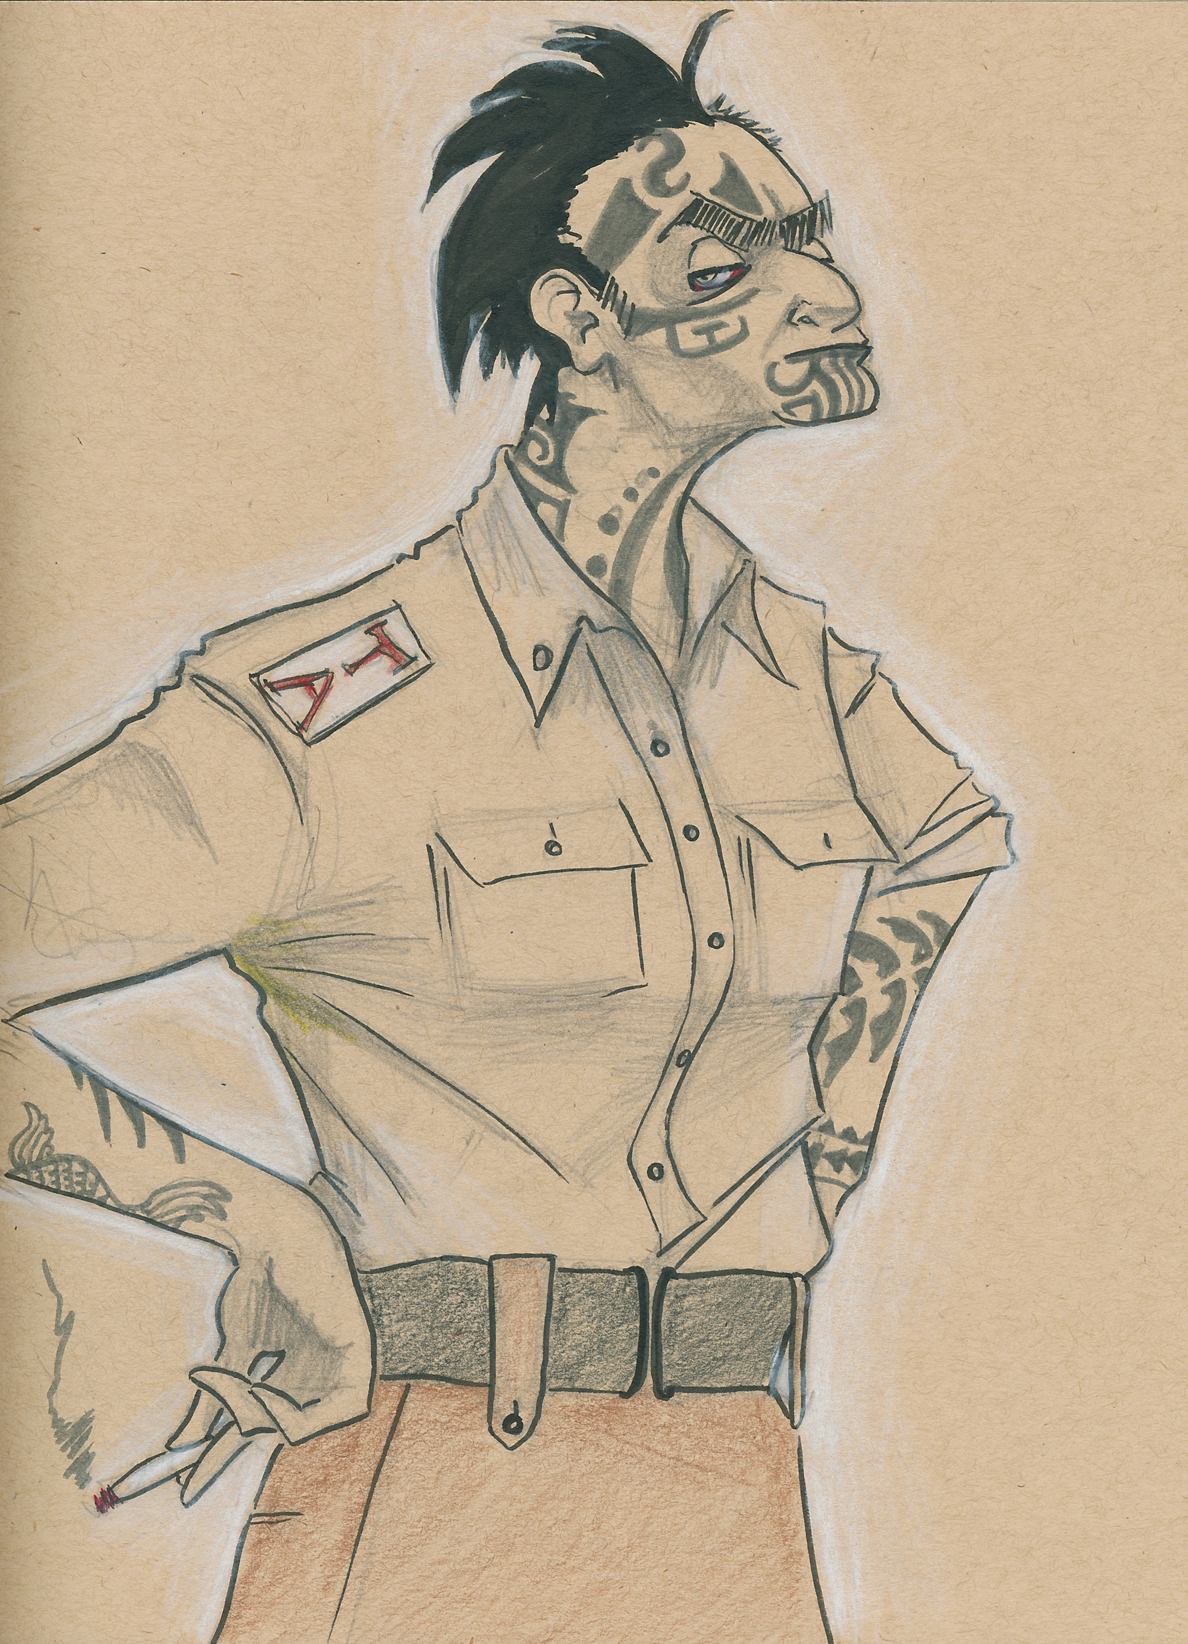
\includegraphics[width=12cm]{img/book1_jaya_misc_tough.png}
\end{center}
\newpage
~